
Question 1 Bilan des Actions Mécaniques Extérieures:

Théorème ou Principe utilisé, éléments d'application :

Équation d'équilibre :

\begin{center}
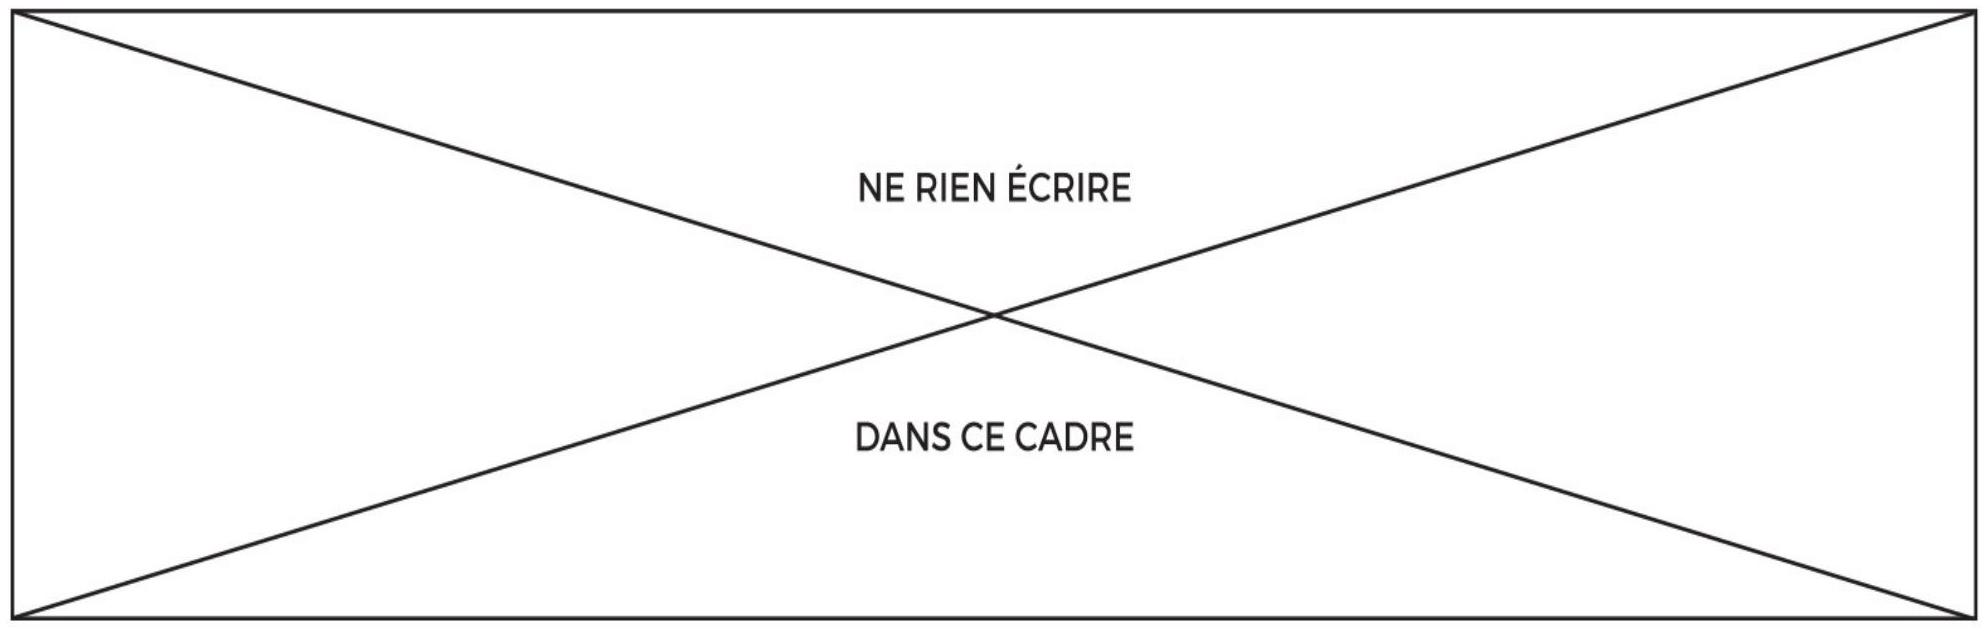
\includegraphics[width=\textwidth]{2024_04_26_3285cfc264024262add0g-21}
\caption{\label{ccmp2023_fig_01}
\end{center}

Question 2

$$
b m_{3}=
$$

Question 3
xxxx
%%%#顷(2)

(4)

\section*{Question 4}
$m_{i}=$

$m_{u}=$

$$
h=
$$

Intérêt de l'hyperstatisme :

\section*{Question 5}
Liaison $(\mathrm{N}) /(5)$ :

Justification :

Liaison $(\mathrm{N}) /(\mathrm{v})$ :

Justification :

\section*{Question 6}
\begin{center}
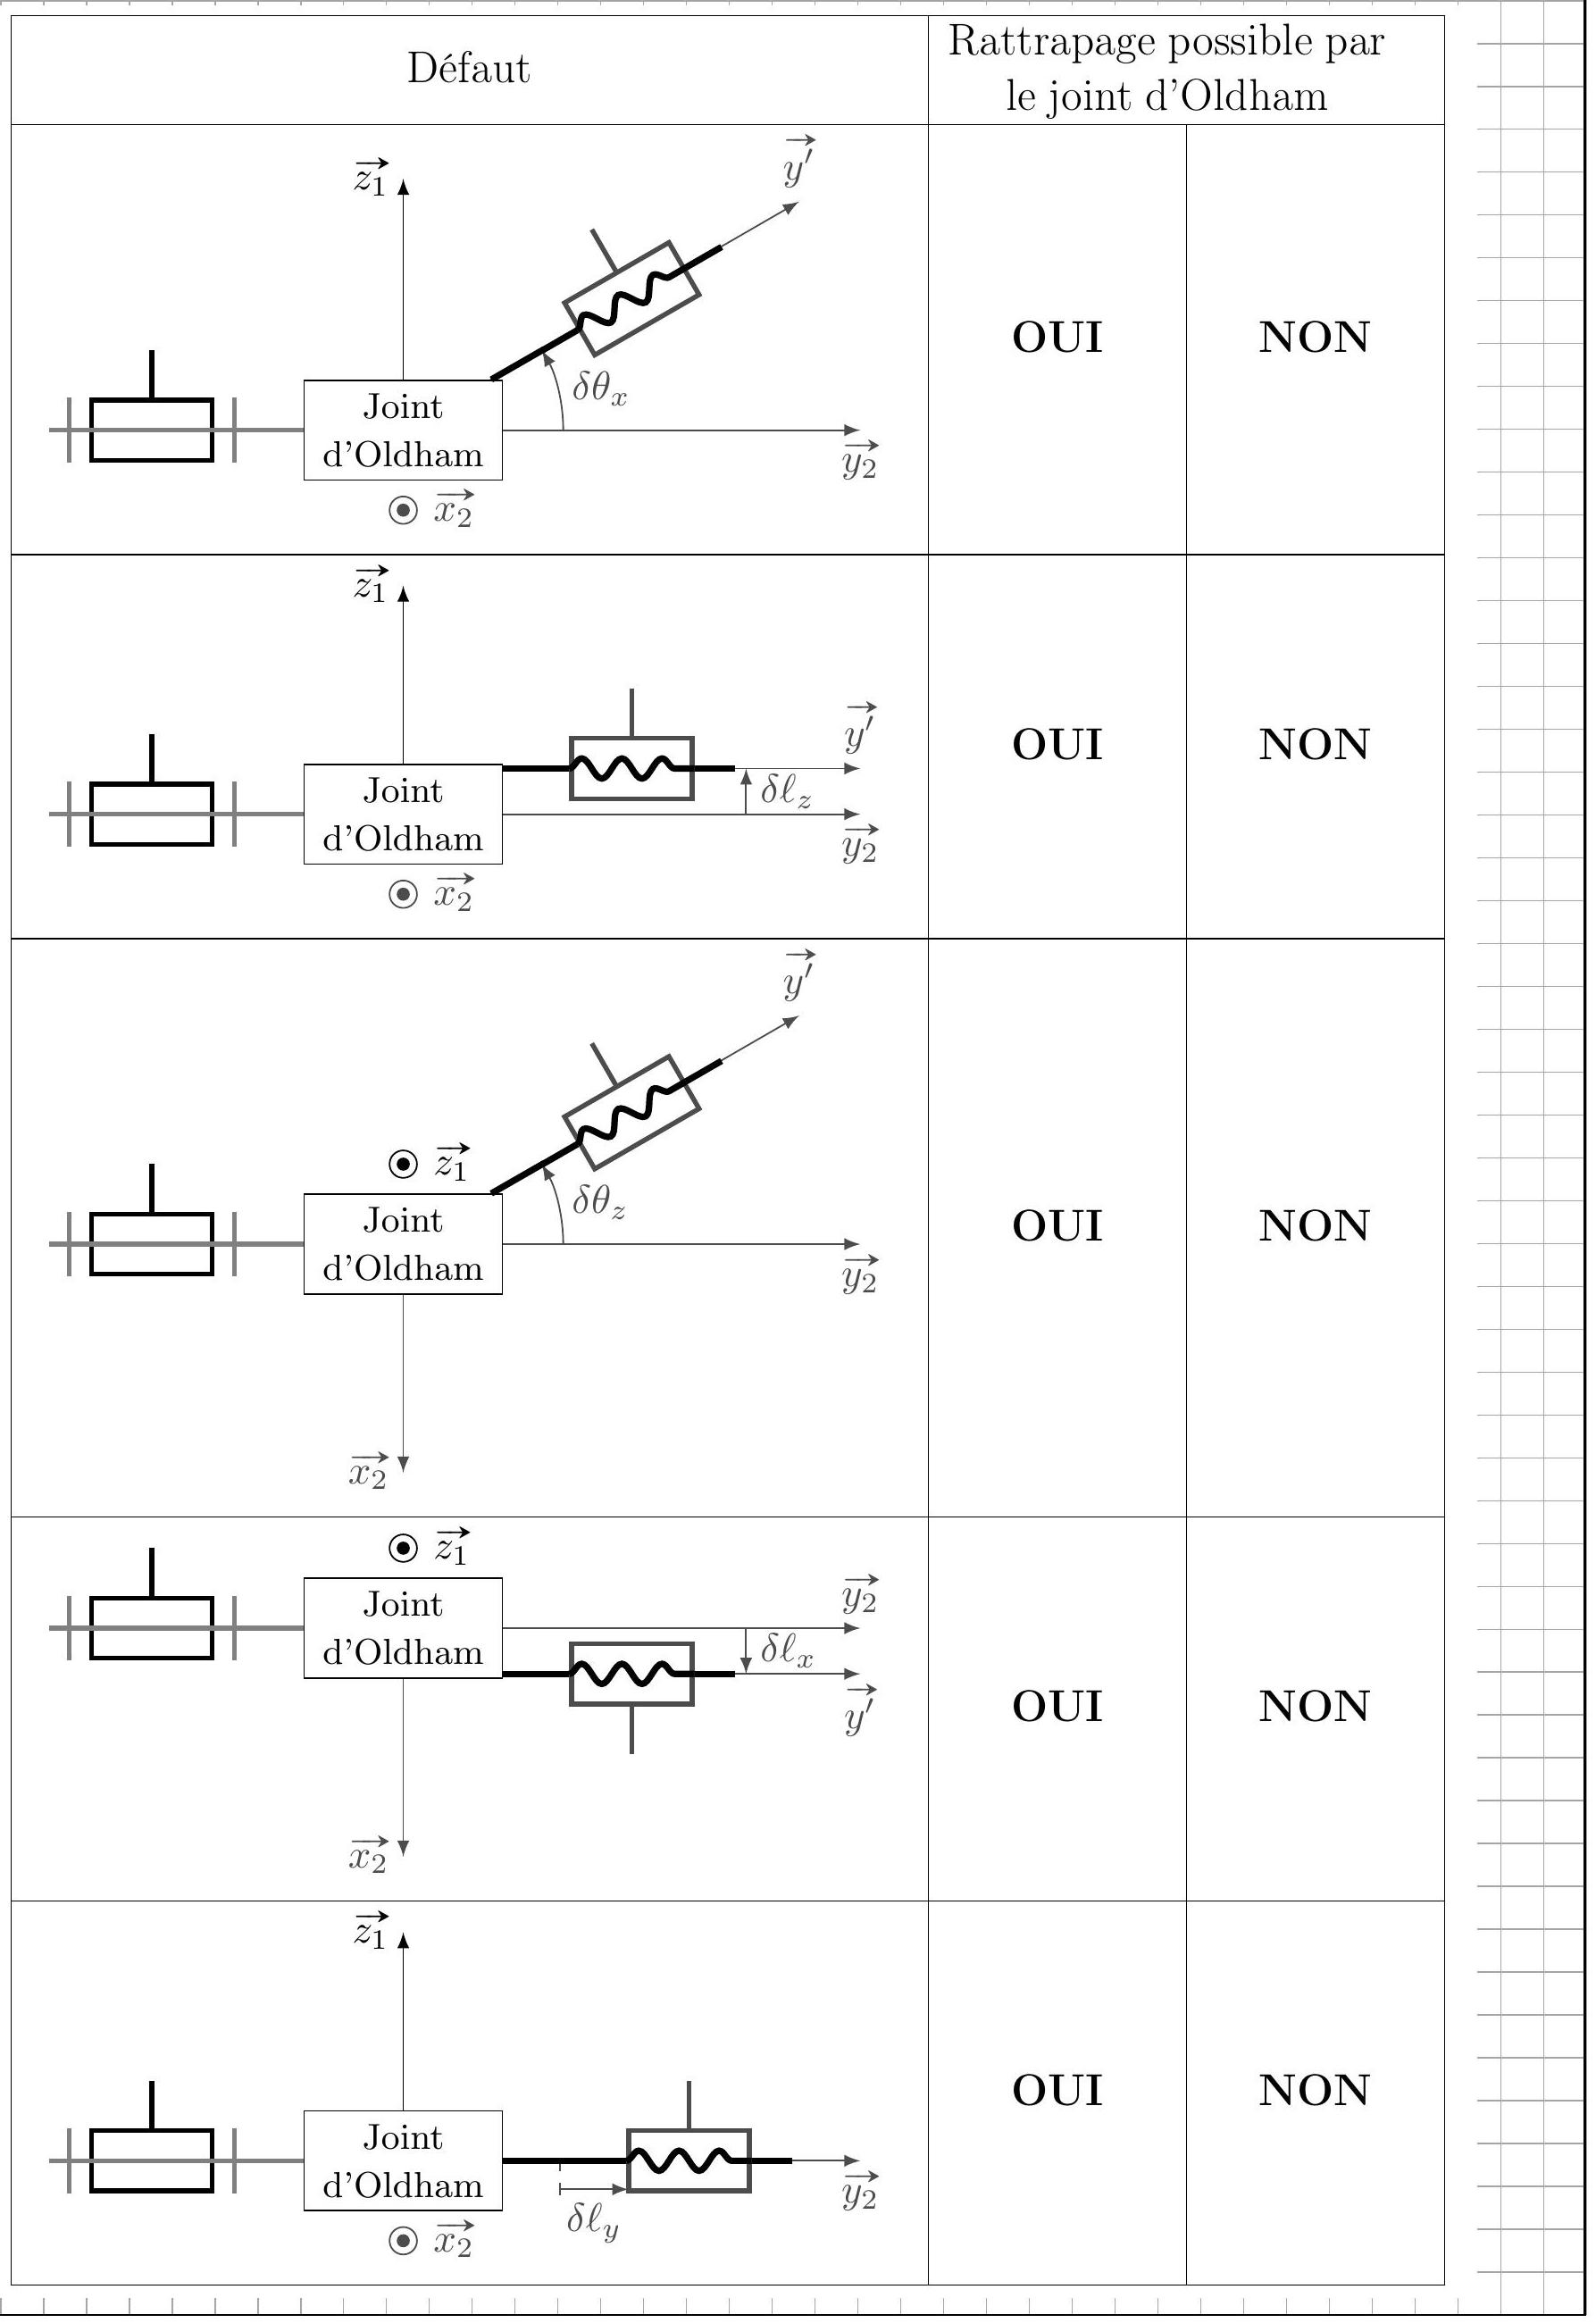
\includegraphics[width=\textwidth]{2024_04_26_3285cfc264024262add0g-23}
\caption{\label{ccmp2023_fig_01}
\end{center}

\begin{center}
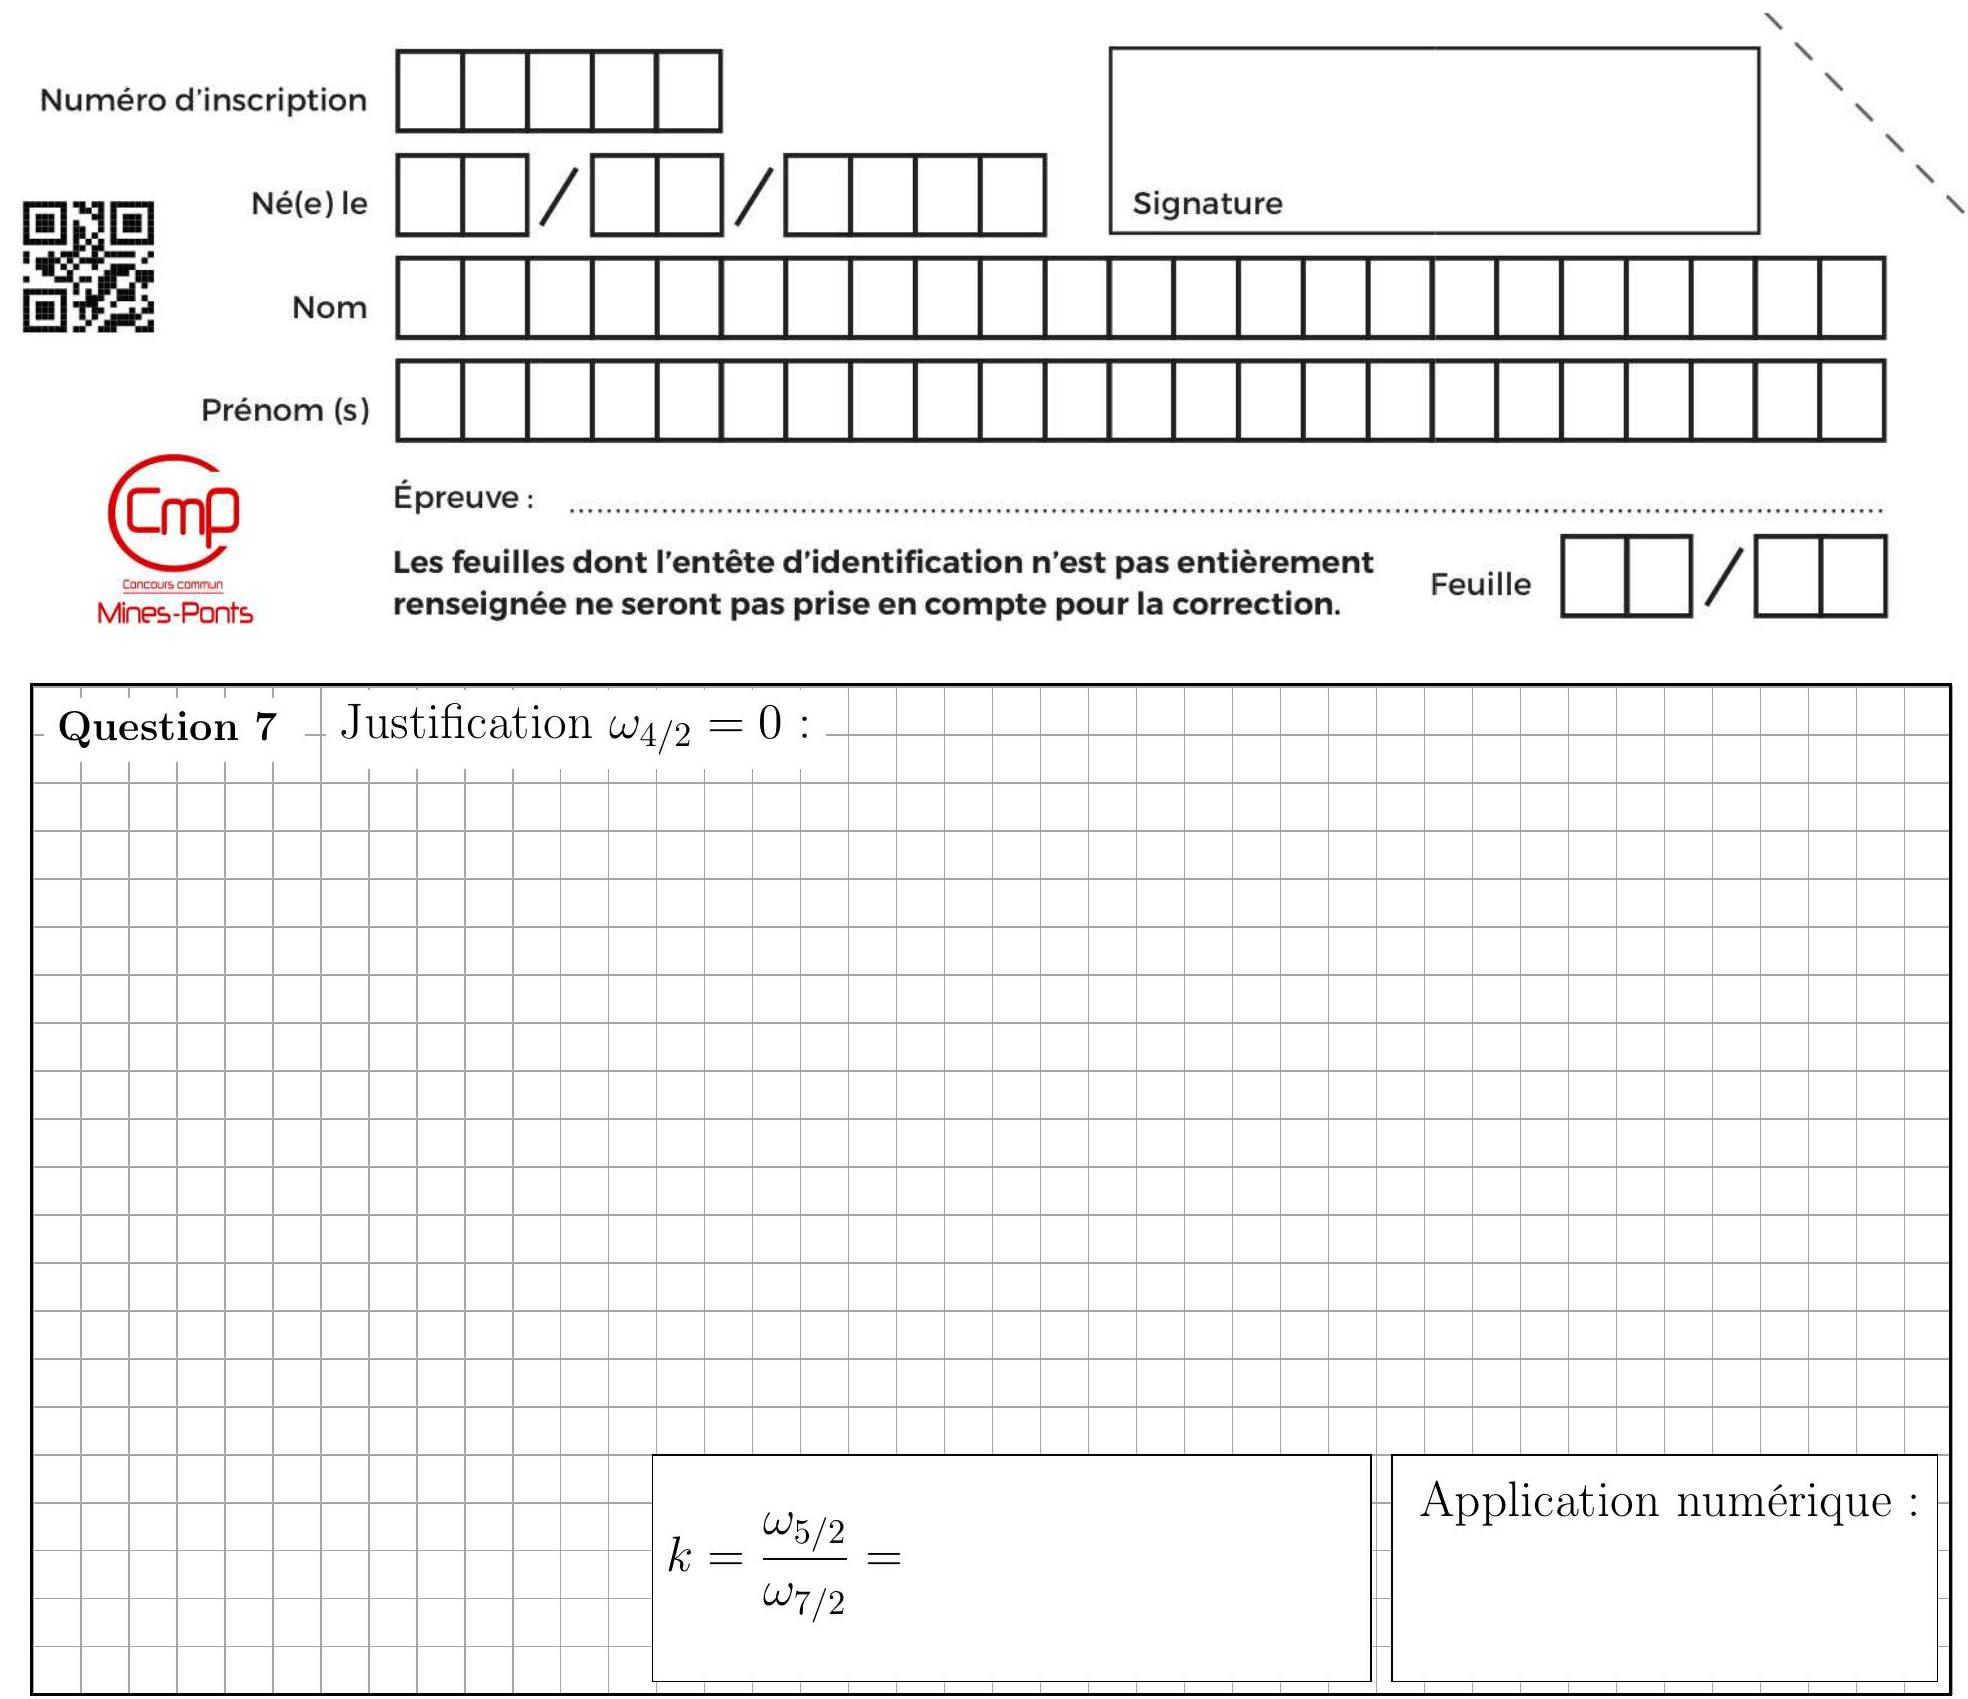
\includegraphics[width=\textwidth]{2024_04_26_3285cfc264024262add0g-24}
\end{center}

\section*{Question 8}
$$
k_{g}=\frac{\omega_{5 / 2}}{\omega_{m / 2}}=
$$

\section*{Question 9}
$d_{v}=$

Application numérique : $d_{v}=$

Conclusion vis-à-vis de l'exigence 1.1 :

\begin{center}
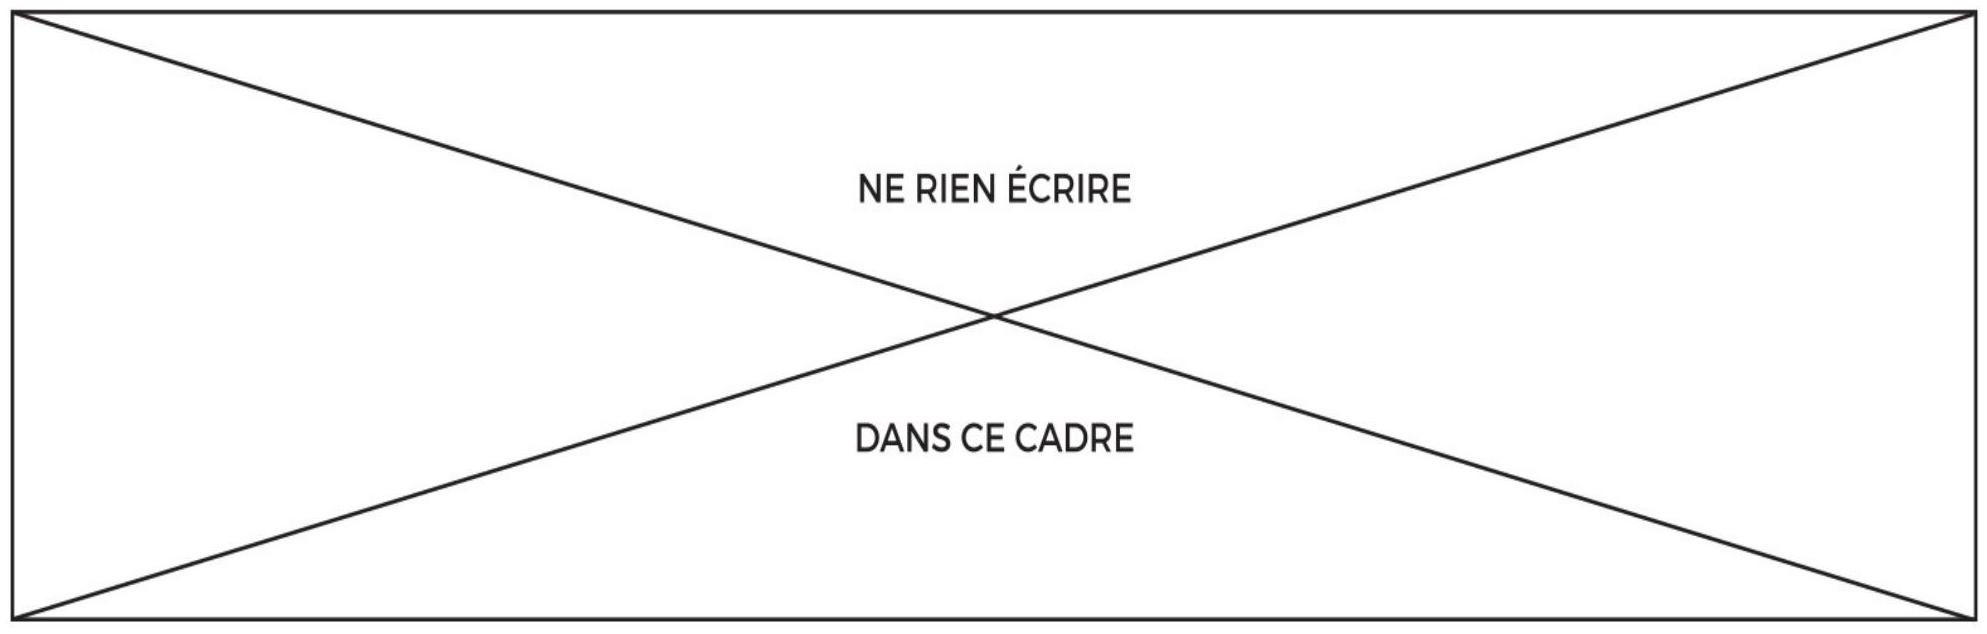
\includegraphics[width=\textwidth]{2024_04_26_3285cfc264024262add0g-25}
\end{center}

Question 10

Question 11

Erreur de positionnement :

Conclusion vis-à-vis de l'exigence 1.1:

Question 12 - Plan de symétrie:

$$
\overline{\bar{I}}_{\left(O_{1}, 2+3\right)}=
$$

Question 13

$\vec{\sigma}_{O_{1},(2+3) / R_{0}}=$

Question 14 Calcul de $\vec{\delta}_{O_{1},(2+3) / R_{0}} \cdot \overrightarrow{z_{1}}$ :

$$
\gamma_{x 2}(t)=
$$

\section*{Question 15}
Système isolé :

Théorème utilisé :

Justification équation non-linéaire :

Question 16

\begin{center}
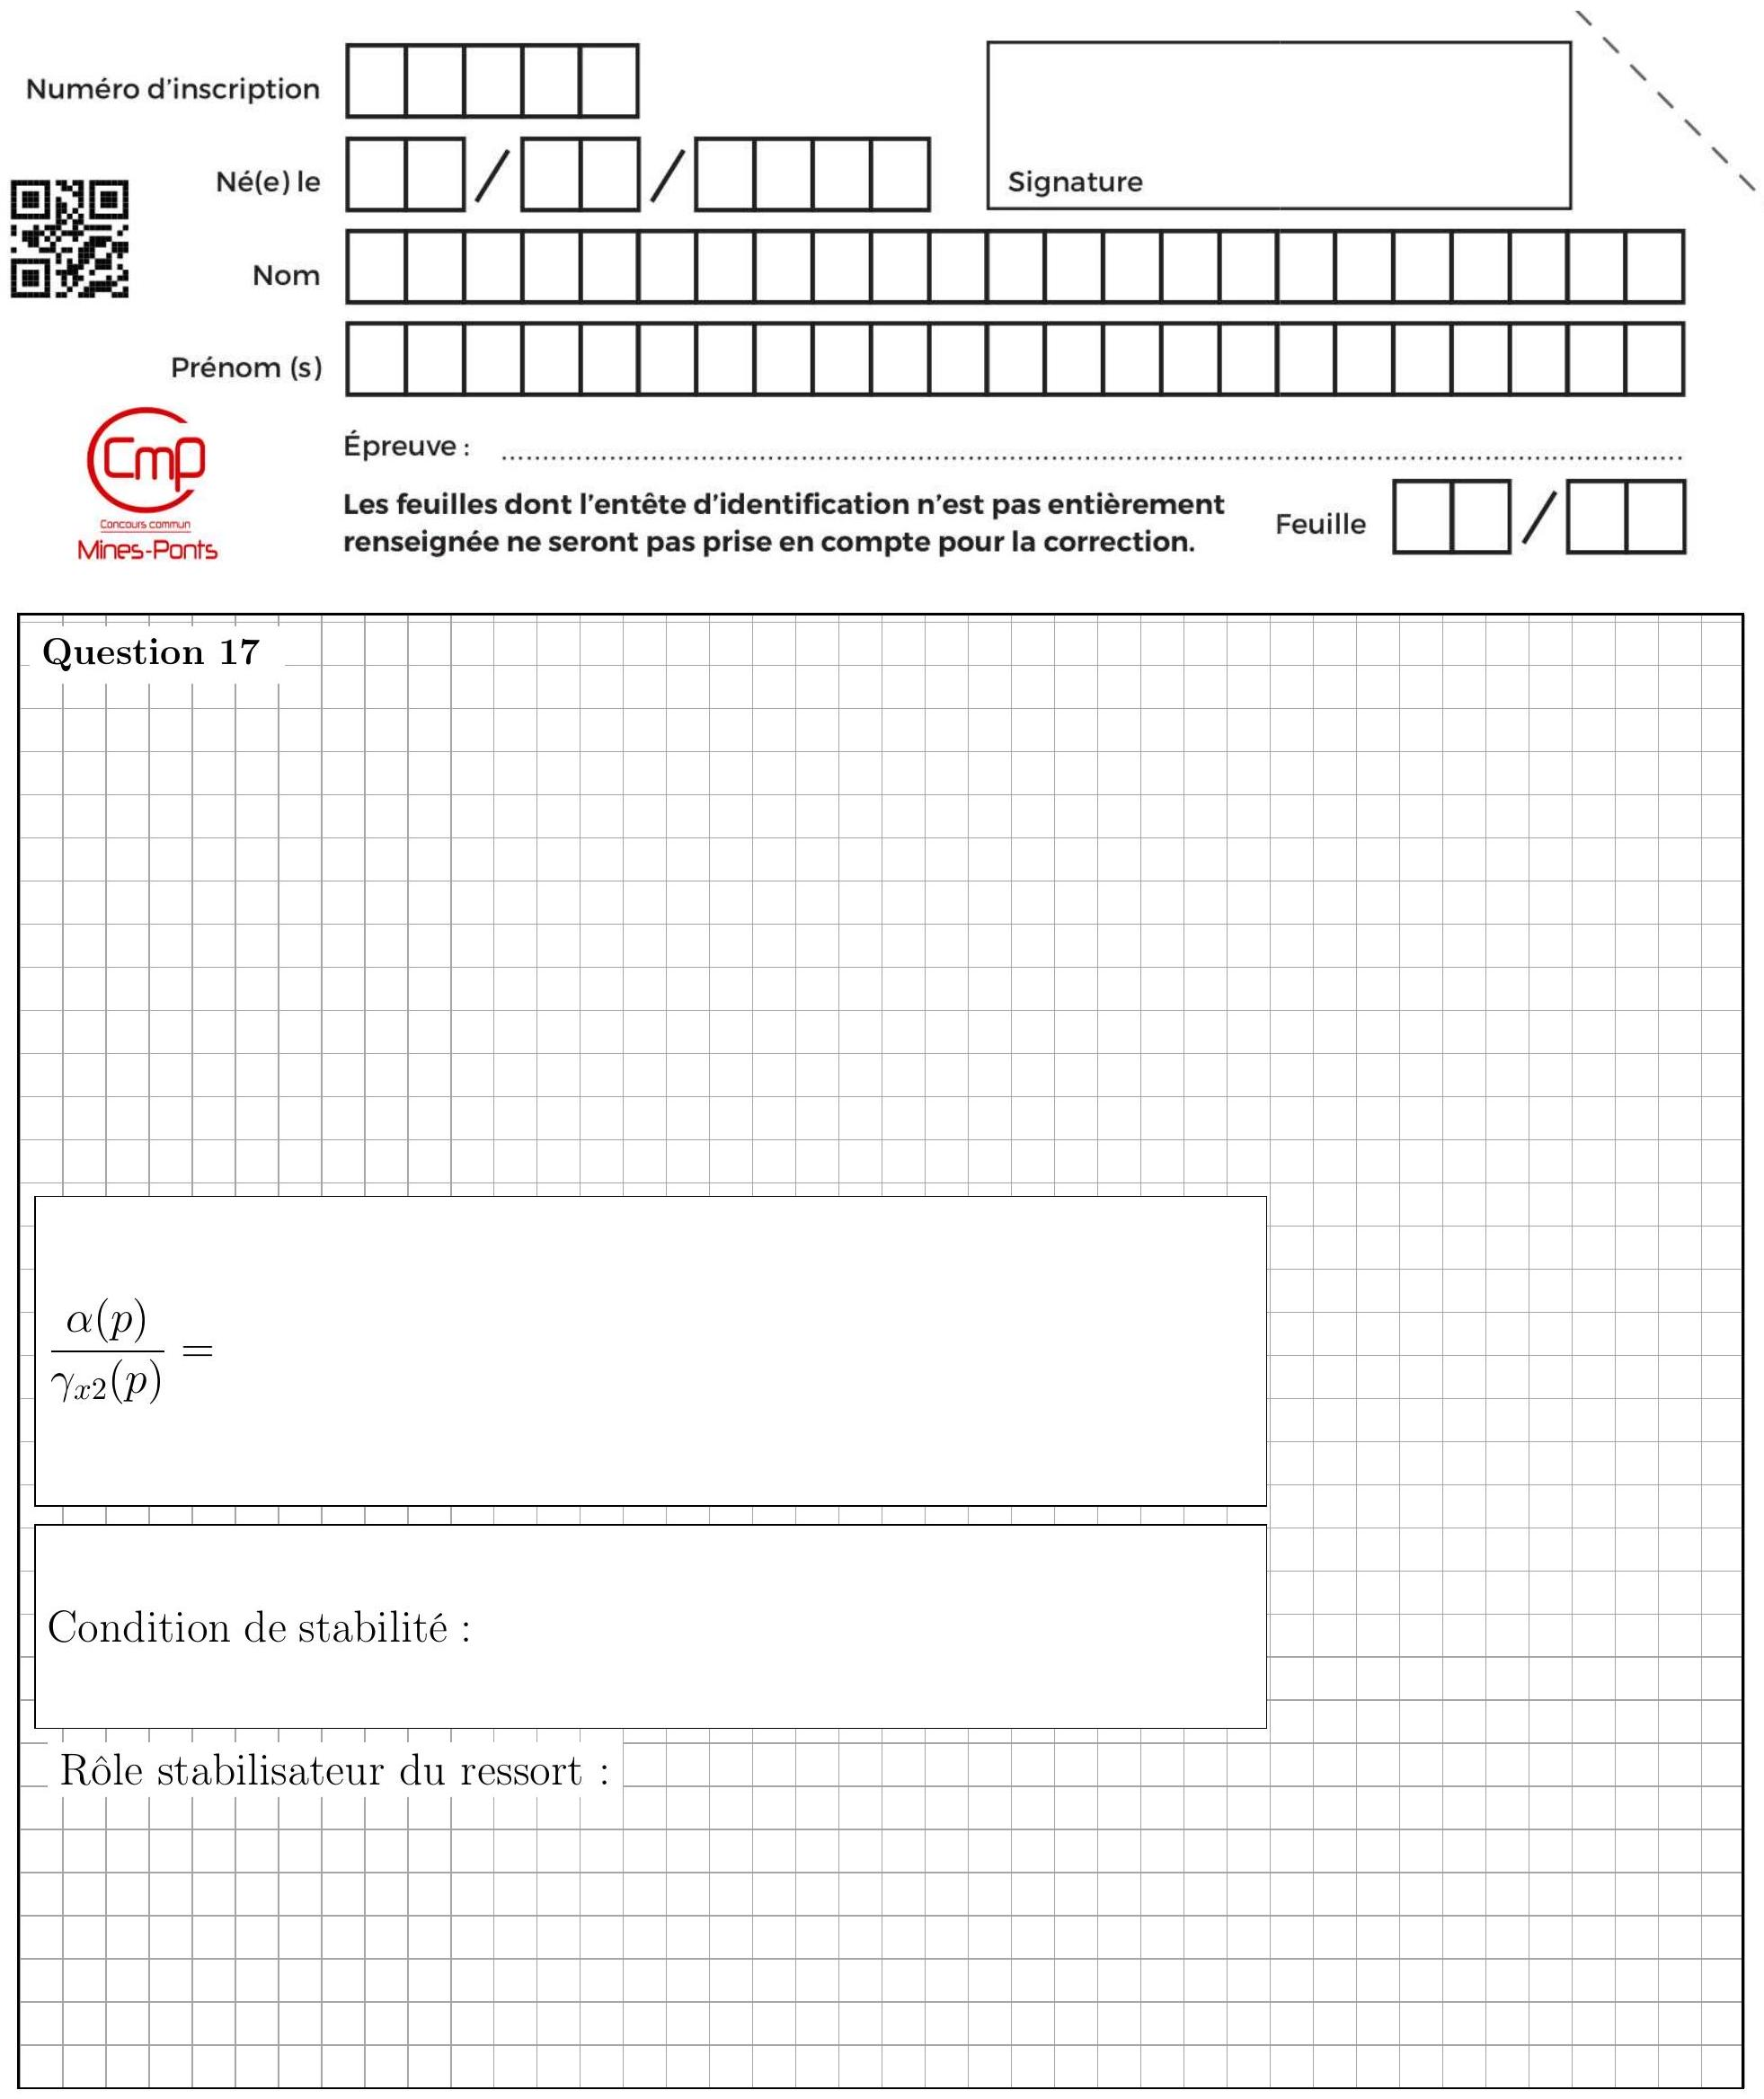
\includegraphics[width=\textwidth]{2024_04_26_3285cfc264024262add0g-28}
\end{center}

\section*{Question 18}
$A=\quad \omega_{0}=\quad \xi=$

\begin{center}
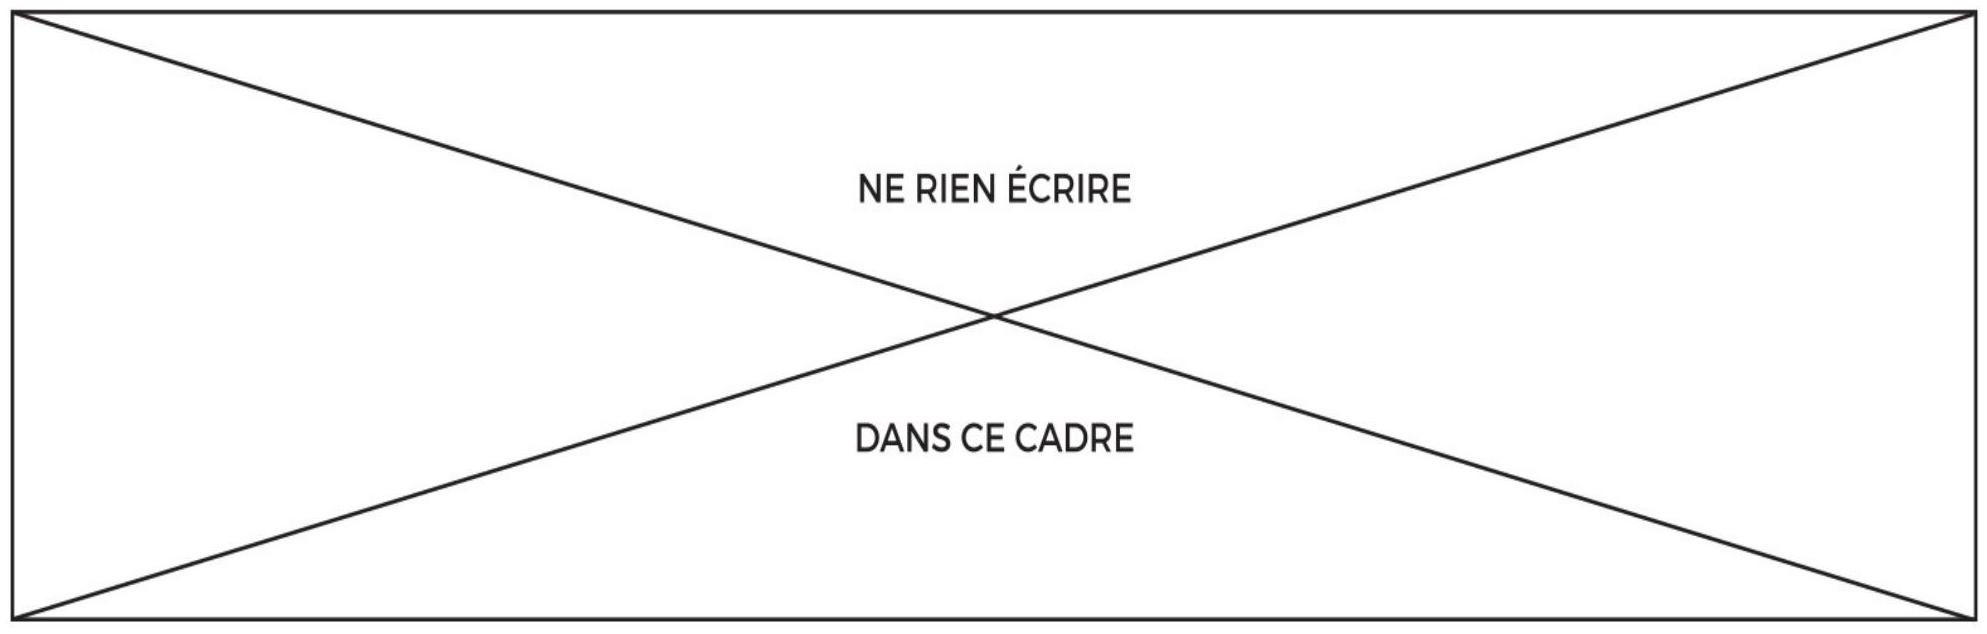
\includegraphics[width=\textwidth]{2024_04_26_3285cfc264024262add0g-29}
\end{center}

Question 19

$C_{0}=$

Question 20

Plage de valeurs de $k$ :

Question 21

\begin{center}
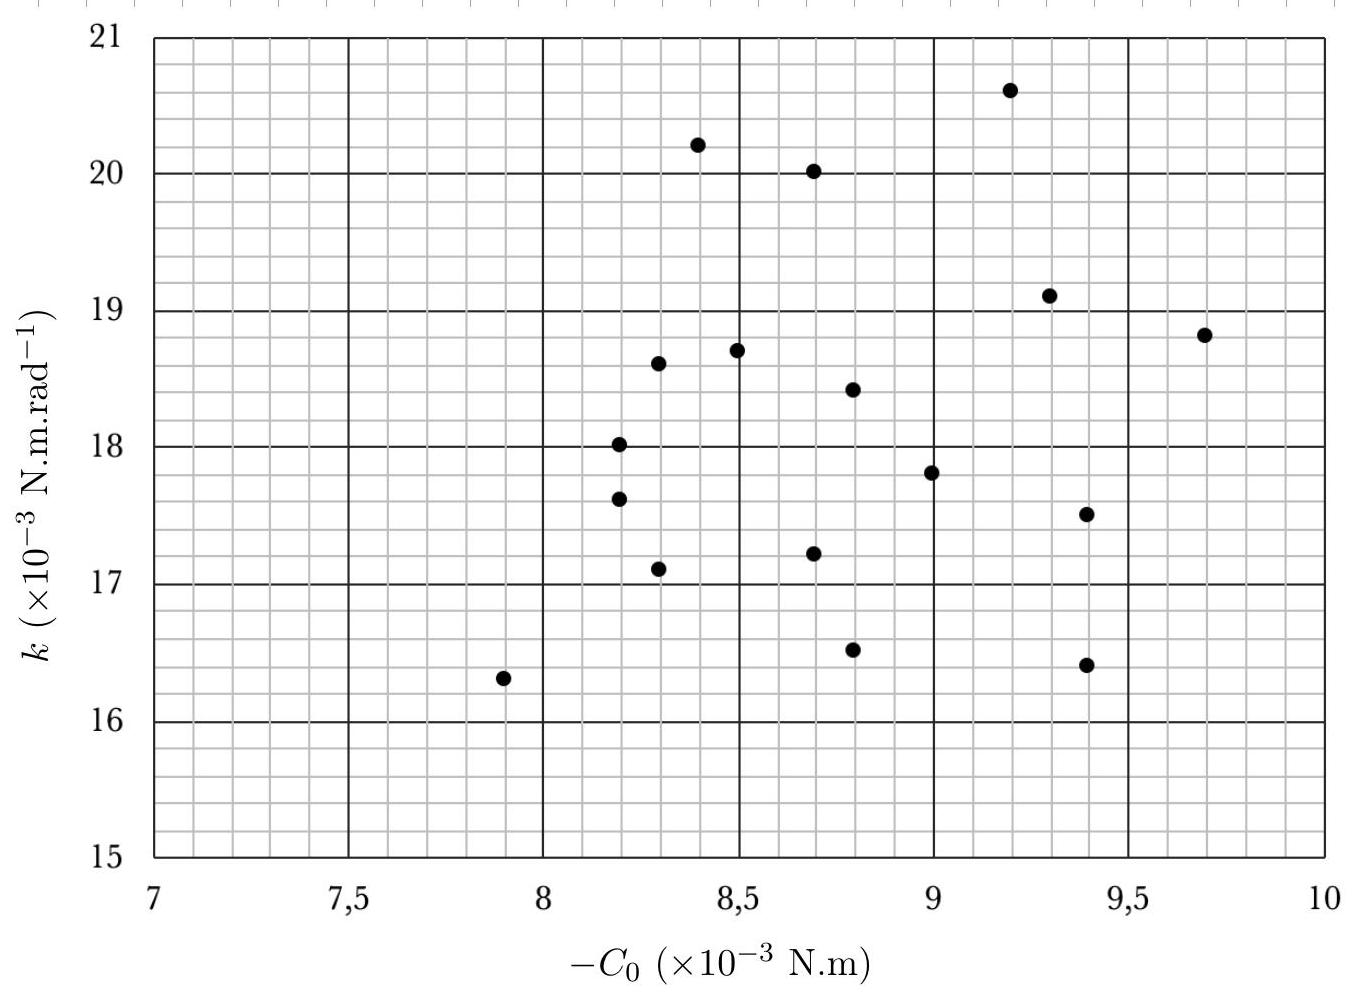
\includegraphics[width=\textwidth]{2024_04_26_3285cfc264024262add0g-30}
\end{center}

Figure A

\section*{Question 22}
\begin{center}
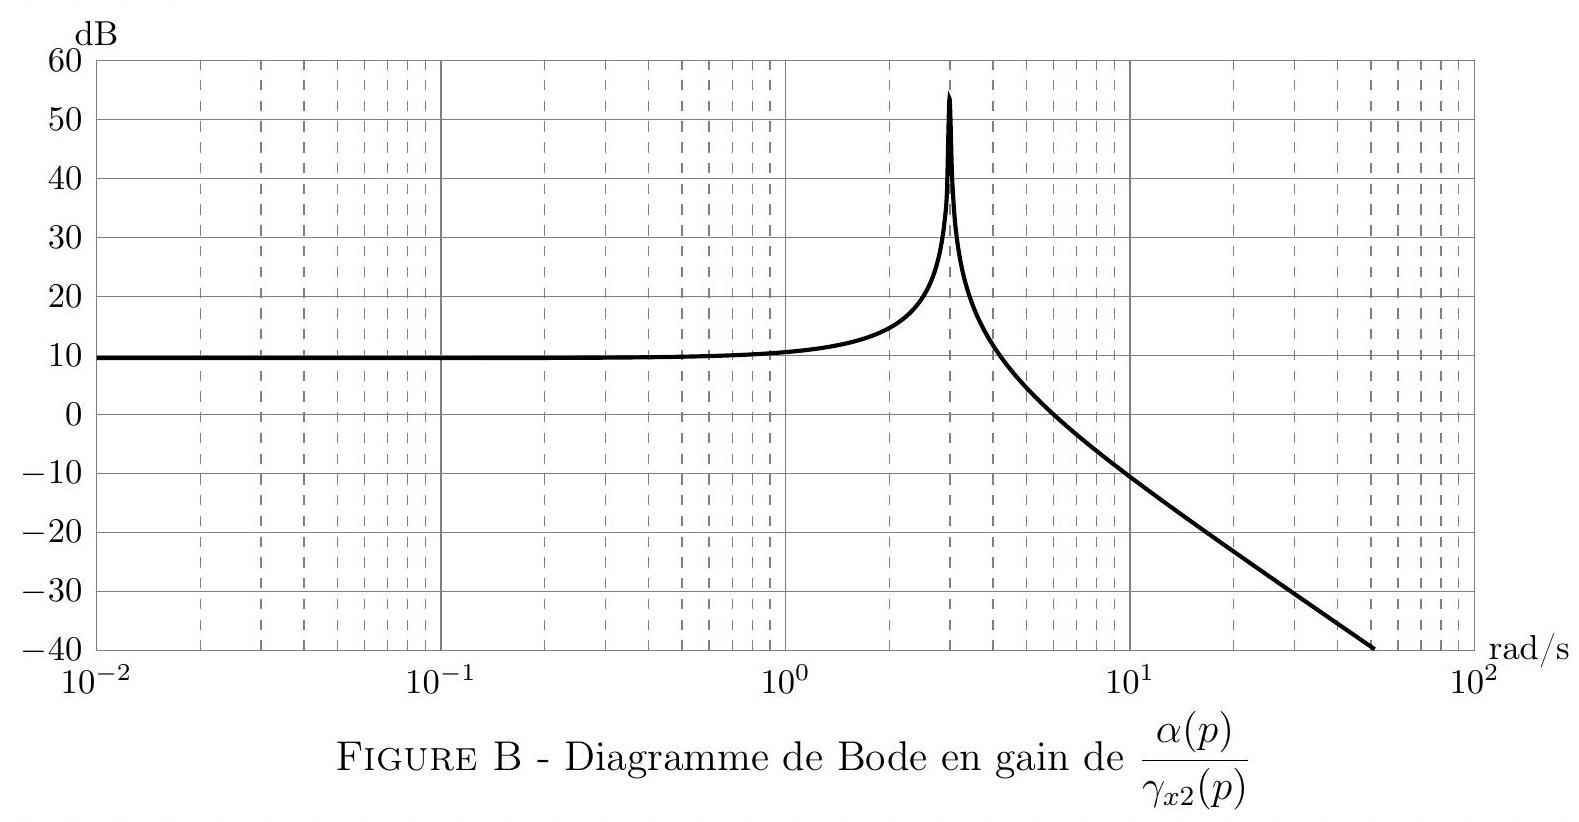
\includegraphics[width=\textwidth]{2024_04_26_3285cfc264024262add0g-30(1)}
\end{center}

Conclusion :

Question 23

\begin{center}
\begin{tabular}{|l|l|}
\hline
$H_{\gamma}(p)=$ \\
\hline
$k_{\mathrm{HF}}=$ \\
\hline
$b_{1}=$ \\
\hline
$b_{2}=$ \\
\hline
$a_{1}=$ \\
\hline
$b_{3}=$ \\
\hline
\end{tabular}
\end{center}

Question 24 - Justification de la stabilité :

\begin{center}
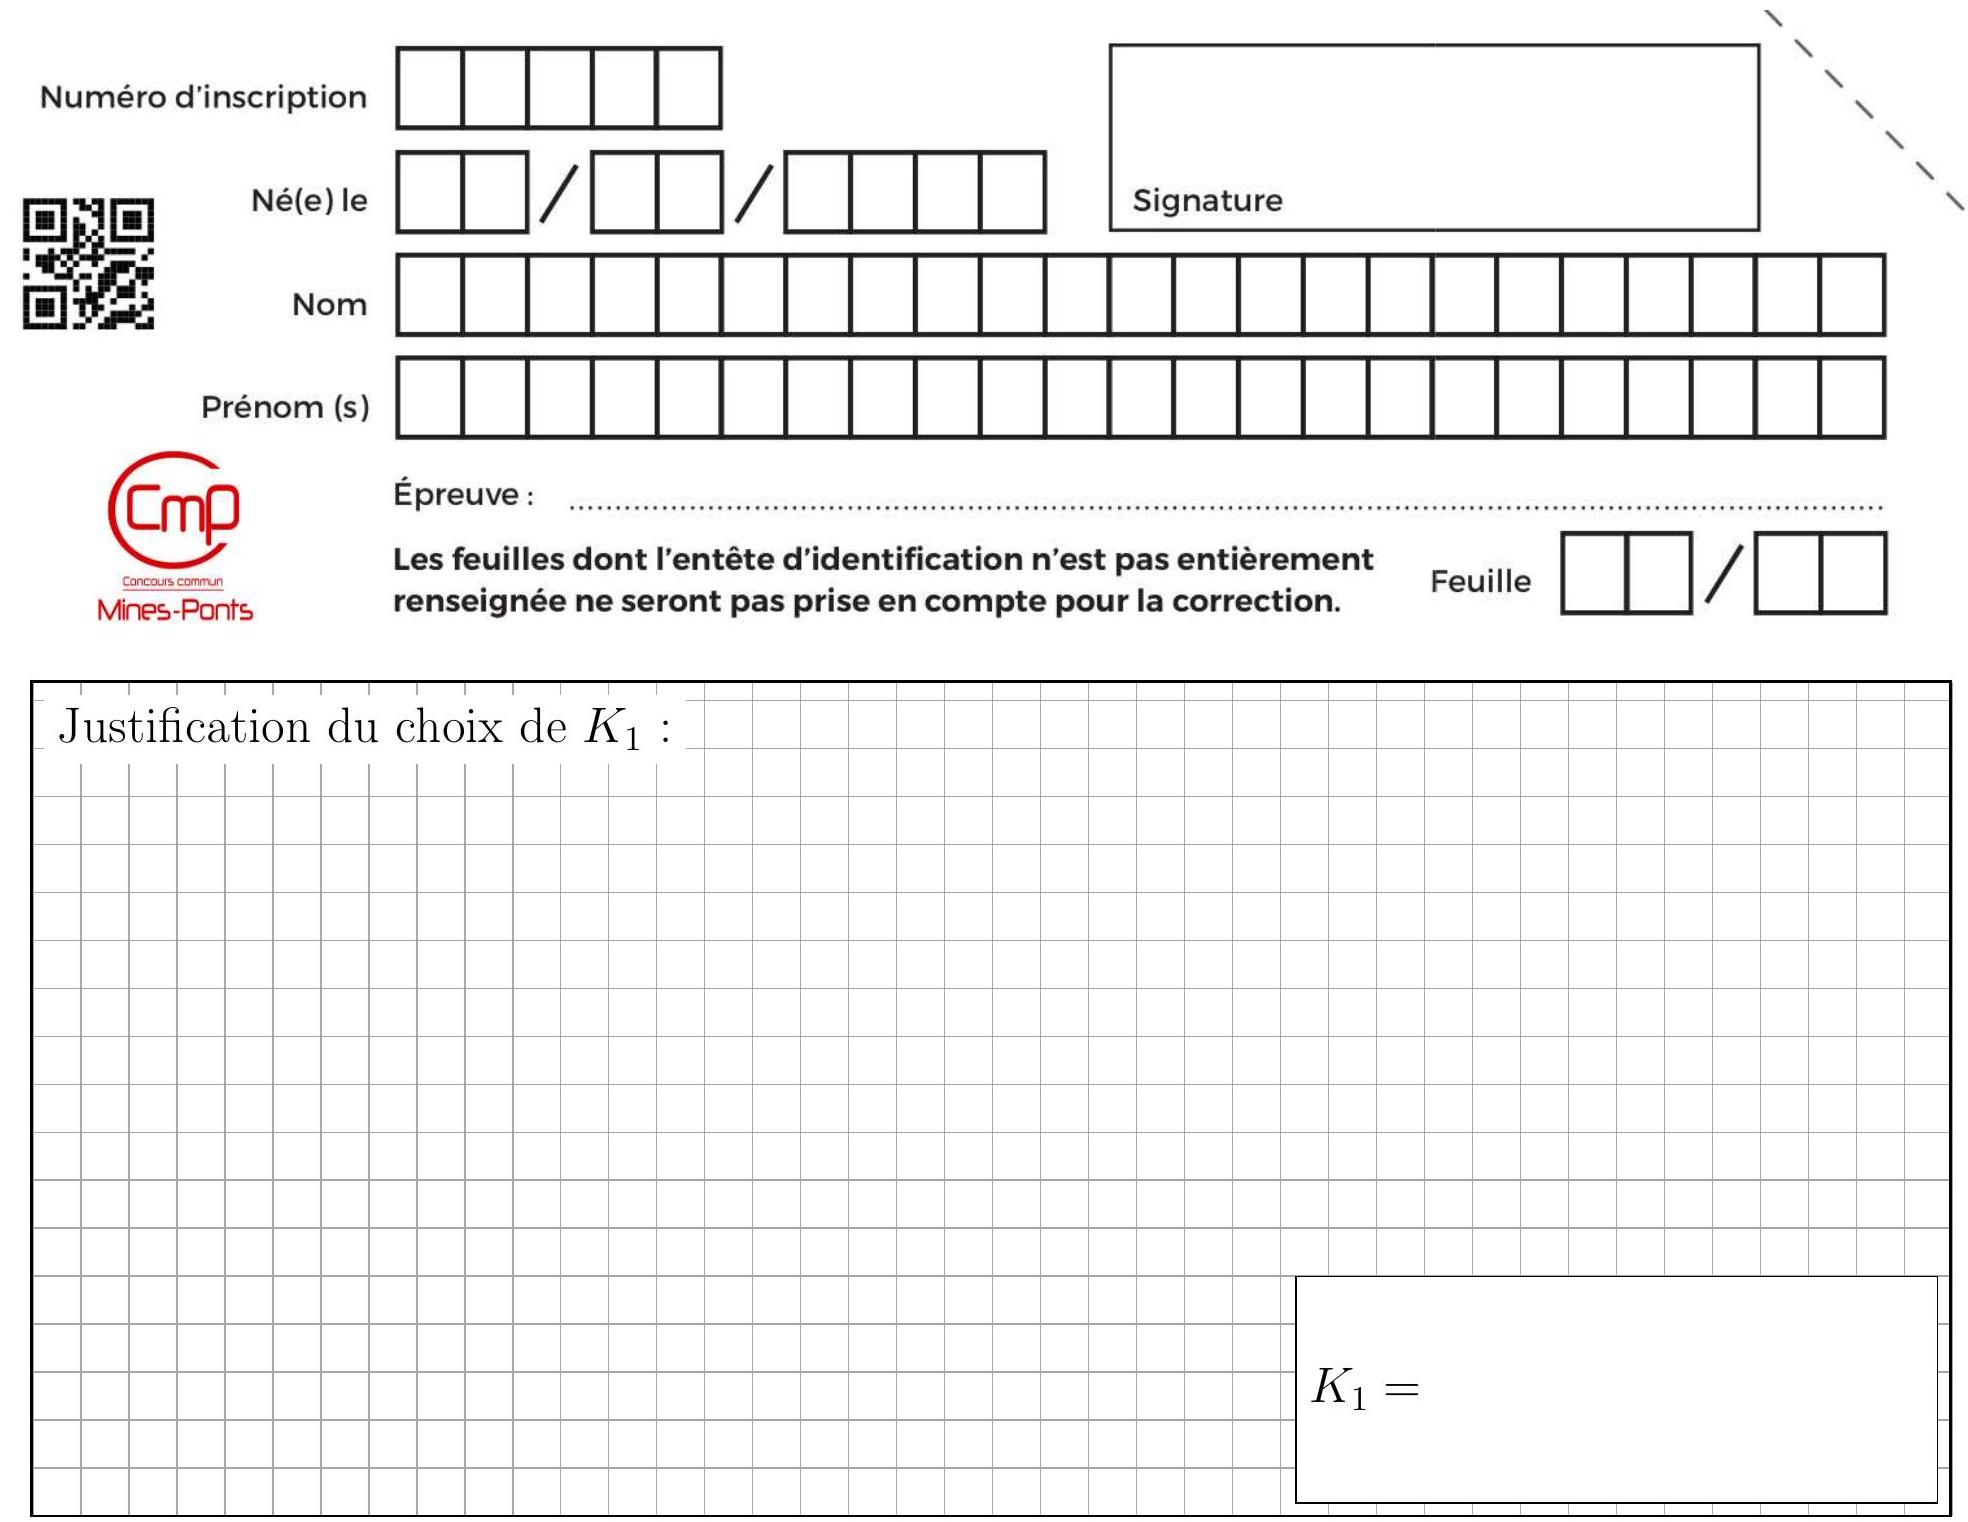
\includegraphics[width=\textwidth]{2024_04_26_3285cfc264024262add0g-32}
\end{center}

Question 25

$\tau_{2}=$

$\tau_{3}=$

\begin{center}
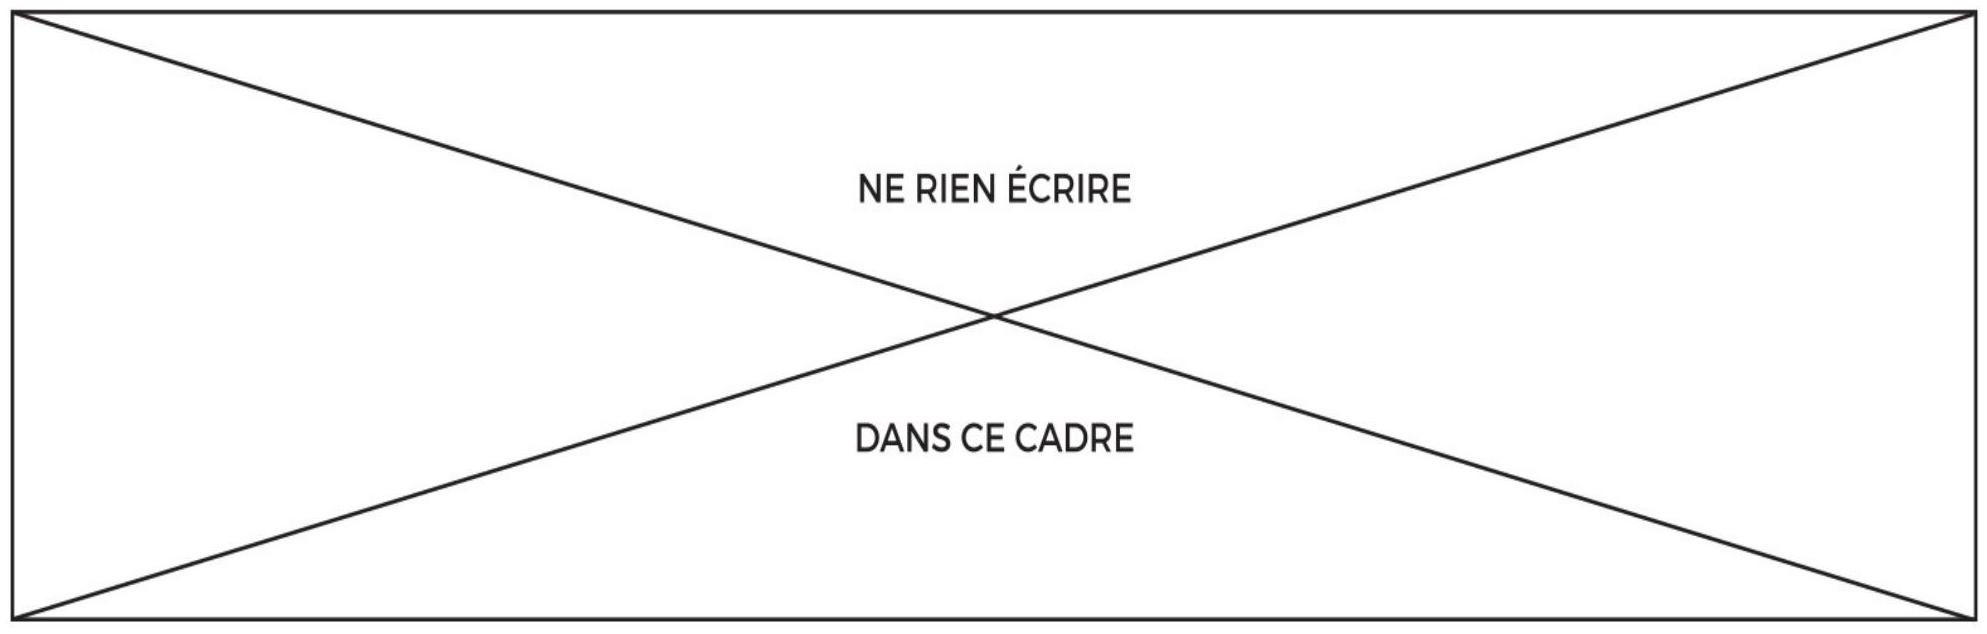
\includegraphics[width=\textwidth]{2024_04_26_3285cfc264024262add0g-33}
\end{center}

Question 26 - Exigence 3.2:

Exigence 3.3 :

Question $27^{-}$Intérêt de la chaîne d'action BF :

Question 28

$$
H_{B O}(p)=
$$

Question 29\\
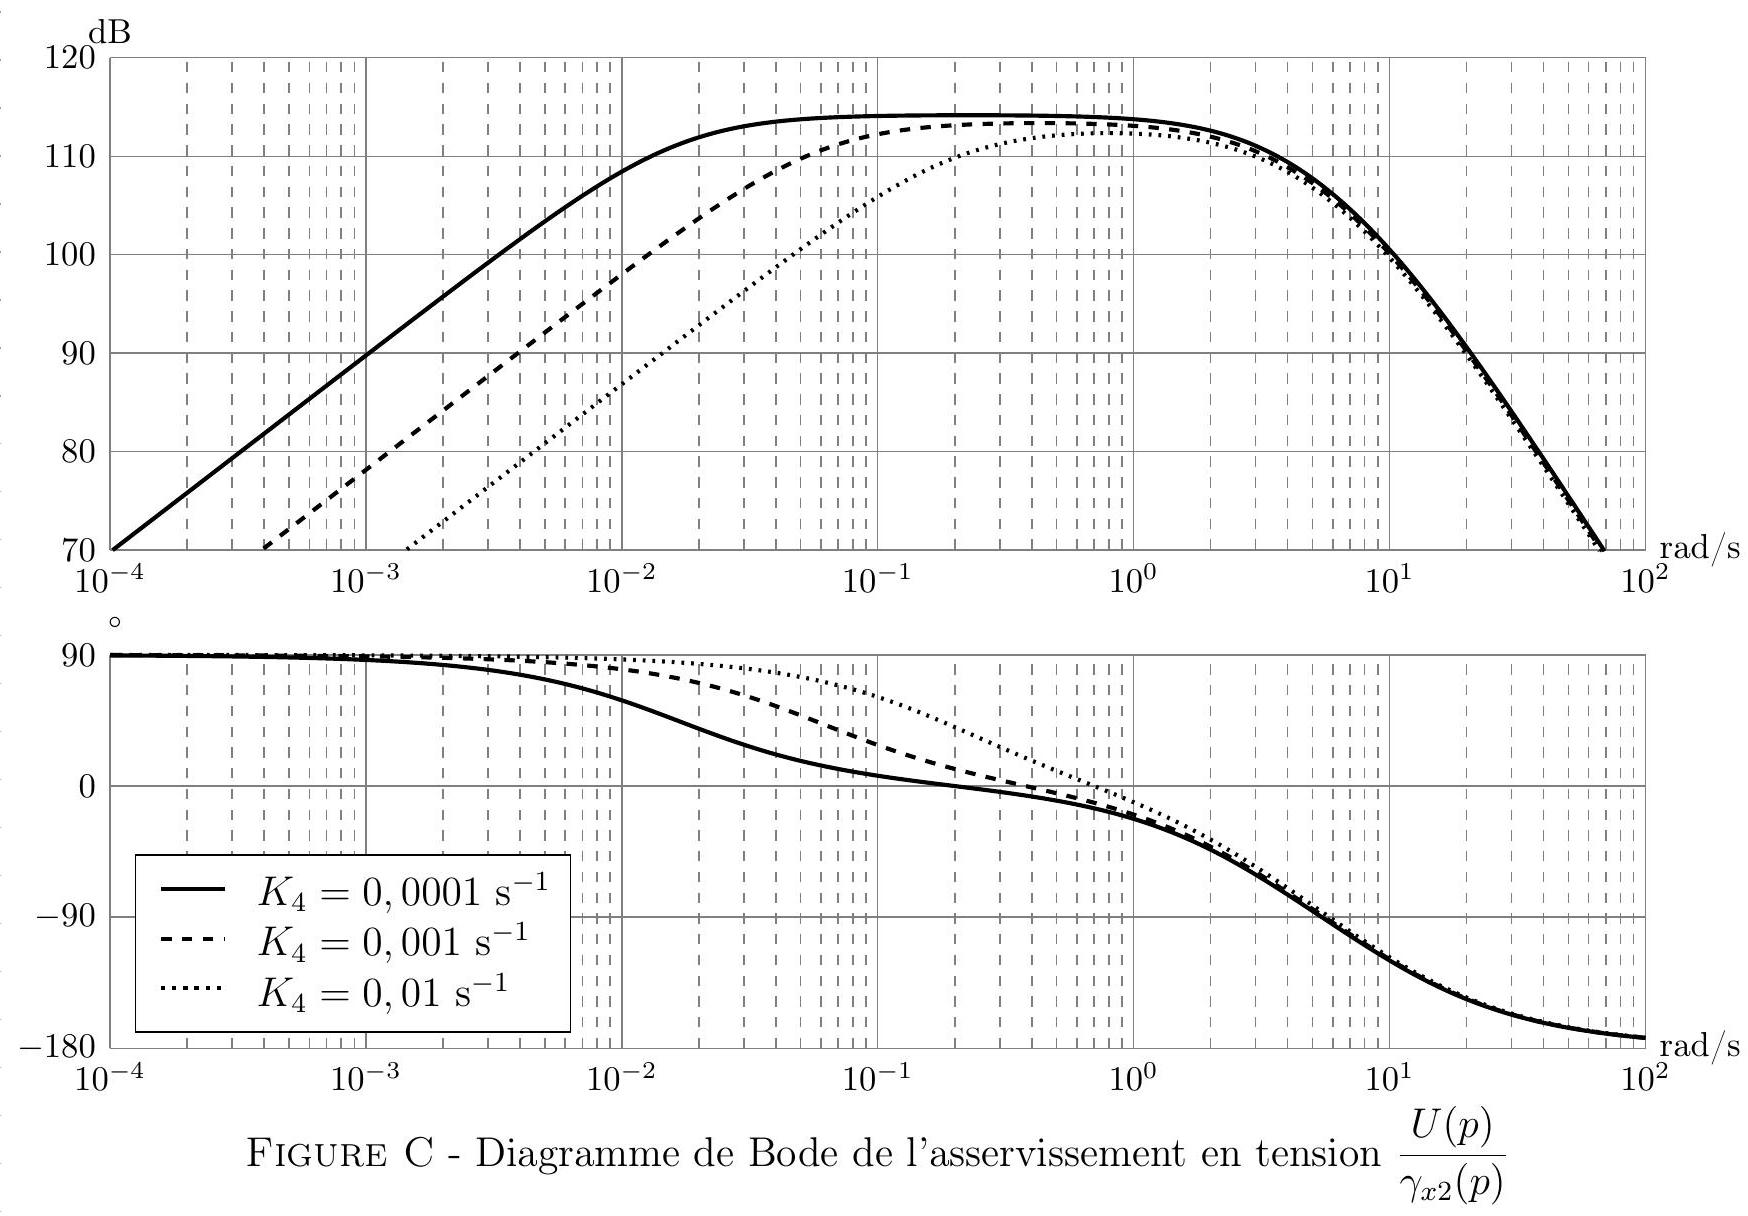
\includegraphics[width=\textwidth]{2024_04_26_3285cfc264024262add0g-34}

$$
K_{4}=
$$

\section*{Question 30}

